% ===============================================
% MATH 373: Intro to Numerical Analysis           Fall 2021
% prog3_testing_template.tex
% June 8, 2021
% ===============================================

% -------------------------------------------------------------------------
% You can ignore this preamble. Go on
% down to the section that says "START HERE" 
% -------------------------------------------------------------------------

\documentclass{article}

% load packages
\usepackage{amsmath,amsfonts,graphicx,amsthm,amssymb,hyperref,xcolor}

% Define default environments
\newenvironment{theorem}[2][Theorem]{\begin{trivlist}
\item[\hskip \labelsep {\bfseries #1}\hskip \labelsep {\bfseries #2.}]}{\end{trivlist}}
\newenvironment{lemma}[2][Lemma]{\begin{trivlist}
\item[\hskip \labelsep {\bfseries #1}\hskip \labelsep {\bfseries #2.}]}{\end{trivlist}}
\newenvironment{claim}[2][Claim]{\begin{trivlist}
\item[\hskip \labelsep {\bfseries #1}\hskip \labelsep {\bfseries #2.}]}{\end{trivlist}}
\newenvironment{problem}[2][Problem]{\begin{trivlist}
\item[\hskip \labelsep {\bfseries #1}\hskip \labelsep {\bfseries #2.}]}{\end{trivlist}}
\newenvironment{proposition}[2][Proposition]{\begin{trivlist}
\item[\hskip \labelsep {\bfseries #1}\hskip \labelsep {\bfseries #2.}]}{\end{trivlist}}
\newenvironment{corollary}[2][Corollary]{\begin{trivlist}
\item[\hskip \labelsep {\bfseries #1}\hskip \labelsep {\bfseries #2.}]}{\end{trivlist}}

\newenvironment{solution}{\begin{proof}[Solution]}{\end{proof}}

%adjust to 1 in margins
  \addtolength{\oddsidemargin}{-.875in}
   \addtolength{\evensidemargin}{-.875in}
    \addtolength{\textwidth}{1.75in}

    \addtolength{\topmargin}{-.875in}
    \addtolength{\textheight}{1.75in}
    
% Define Shortcuts
\def\ds{\displaystyle}
\def\beginrefs{\begin{list}%
        {[\arabic{equation}]}{\usecounter{equation}
         \setlength{\leftmargin}{2.0truecm}\setlength{\labelsep}{0.4truecm}%
         \setlength{\labelwidth}{1.6truecm}}}
\def\endrefs{\end{list}}
\def\bibentry#1{\item[\hbox{[#1]}]}

\begin{document}



% ------------------------------------------ %
%                 START HERE             %
% ------------------------------------------ %

\large

{\Large Math 373, Introduction to Numerical Analysis}

\begin{center}
{\Large Author: \hfill Amanda Lauen} % Replace "Author's Name" with your name
\end{center}
\par \medskip \par
{\Large Programming Assignment: 3} 
\par \bigskip \par

% Complete summary and remove the instructions in red
{\bf Summary:} {\color{black} This assignment states to construct a MATLAB program that calculates an approximation of the total work done by the force.  This program is based on Steven Chapra and Raymond Canale’s work [CC10].  To calculate the approximation and flag, the program will take in force, position, and angle values. It will then determine which rule to use to calculate the approximation based on several checks done.  The methods used in the program include Simpson’s 3/8th Rule and Trapezoidal Rule.  Both rules are detailed in the Tea Time Numerical Analysis textbook [LB16] and Dr. Kyle Riley’s Class Notes and Lectures [KR21].} 
\par \bigskip \par

% Complete methods and remove the instructions in red
{\bf Methods:} {\color{black}       The possible outcome of this program is a flag value indicating an error or a valid process of code, including an approximation of the work done by the force.  The first possible outcome of running this program is an approximation value of -99 with a flag value of 1, indicating that the size of the vectors is not the same.  Another outcome is that an approximation value will be returned along with a flag of 2, indicating that the problem was solved using Simpson’s 3/8th Rule.  The outcome can be an approximation value with a flag value of 3, indicating that the problem was solved using the Trapezoidal Rule. For this code, no additional flags were added.  This code should only return the output variables and should not output or print anything else.  
\par \bigskip \par
The way to make sure this code is effective is to run the code as it is with given values and check them by hand to make sure that the values match.  In this code, Simpson’s 3/8th Rule required uniform spacing.  How I checked that in my code was by setting a y-value equal to diff(x), and then before running the code for Simpson’s 3/8th Rule, I checked if the max of y equals the min of y and then if the absolute value of max(y)=min(y) is less than 10\textsuperscript{-12}. I chose this number because it is small enough to ensure that Uniform Spacing is present and that the code runs effectively.  My code accommodates non-uniform spacing by checking the three conditions of Simpson’s Rule in the initial if statement. If any of the three (even just one) misses, including non-uniform spacing, it goes to the else statement with the Trapezoidal Rule.
 }
\par \bigskip \par


% Complete testing and analysis, please remove the instructions in red
{\bf Testing and Analysis:} {\color{black} I tested my program by hand, calculating specific values within the formulas to approximate the work done by force.  I then calculated the exact value to see if they were within range of one another before putting in these numbers in MATLAB to check if my code was coming up with the same values.  An example of this is when $F(x)=\frac{x}{3}$, $q(x)=\frac{5}{x+0.01}$.  I defined the points of the path as a=0 and b=10.  Afterward, by having a total of n=5 points, I defined the vector of the x-position as $x=[0,2,4,6,8,10]$.  I then evaluated the force and angle at each point x to obtain a table.  After creating the table, I plugged in the values calculated into Simpson’s 3/8th Rule to get the answer.  I then plugged the values into the original integral to get the exact value.  Since I only used n=5 points, the approximation and exact value values are close but not equal.  If I increase the number of points, the error will reduce.  More about this example, other examples, and the code work will be shown in the Appendix.  
\par \bigskip \par
In terms of negative values of work, it is possible to obtain them.  Negative work refers to a situation in which the direction of force is opposite to the direction of motion.  An example of this is work done by friction.  Mathematically, the function integrated is: $F(x)cos(\theta(x))$.  The value of F(x) (its magnitude) is always positive. However, the function $cos(x)$ varies between -1 and 1, which means that for values of $\theta$ in the domain $(\pi/2,3\pi/2)$ will result in $cos(x)$ being negative.  Negative work implies that the force tends to slow down.  If it was a moving object, then the object’s force slows down, meaning a decrease in its kinetic energy.
\par \bigskip \par
It is advantageous to use Simpson’s 3/8th Rule over the Trapezoidal Rule because Simpson’s 3/8th Rule has a higher degree of accuracy than the Trapezoidal Rule.  Simpson’s 3/8th Rule gives a more accurate result when compared to Simpson’s 1/3rd and Trapezoidal Rules.  This notion helps in knowing what the actual value is versus just having an approximation.  Even though Simpson’s 3/8th Rule has more significant computational effort than Trapezoidal, it still can produce a more accurate approximation than the Trapezoidal Method.
 
\par \bigskip \par
}
%Hit list is optional, but is evidence of higher learning, developing strong skills in reviewing are extremely valuable. Please remove instructions in red.
{\bf Hit List}: {\color{black}
At the time of writing this report, I do not see any errors with my code.  If side cases were neglected, I would have liked to know which ones and code them into my program correctly.  If any errors are to come up with this code, it would only be the errors with the indicated flag and approximation that is defined within the code.
\par \medskip
If I had more time to work on this program, I would have liked to delve into these two methods of finding the work done and if Simpson’s 1/3rd Rule would be able to calculate the work done.  It would have been interesting to compare all three methods to see the differences between them when calculating the work done by the force, position, and angle given by the user.}

\par \bigskip \par

%Integrity Statement Leave the statement in red and follow it with ``I affirm that this program submission complies with the integrity specifications of this assignment. I understand if I am in violation of the integrity specification then I will get a zero on the assignment and receive an overall reduction in my course grade by one letter grade. ``

{\bf Academic Integrity}: {\color{black} The goal of this assignment is that everyone write their own code. This means you should not copy any code from any other source (the only exception are the templates provided by the instructor.) If you copy any code then you are in violation of integrity specifications of this assignment. If you provide your code to others then you are also in violation of the integrity rules of this assignment. 

I affirm that this program submission complies with the integrity specifications of this assignment. I understand if I am in violation of the integrity specification then I will get a zero on the assignment and receive an overall reduction in my course grade by one letter grade.}

% Add references here, list alphabetically according to last name of primary author.
\section*{References}
\beginrefs


\bibentry{LB16}{\sc Leon Brin},
{\it Tea Time Numerical Analysis (Experiences in Mathematics)  (2nd ed.)}, 2016. Website: \href{http://lqbrin.github.io/tea-time-numerical/}{lqbrin.github.io/tea-time-numerical} .


\bibentry{CC10}{\sc Steven Chapra} and {\sc Raymond Canale}, {\it Numerical Methods for Engineers (6 ed.)}, 2010.

\bibentry{KR21} {\sc Kyle Riley}, Class Lecture, Math 373: Introduction to Numerical Analysis, Lecture, August 2021. 

\endrefs

\bigskip \par \bigskip
%%%------------------------------------------------------
%  Appendix, remove the red comments when completing this section. 
%%----------------------------------------------------------
{\Large {\bf Appendix}} \par \medskip


{\color{black}
 As stated in the Testing and Analysis portion of this report, I tested this program by first defining functions of force, an angle function, and an x-value and calculating them by hand to get the approximation and exact value and compare them to the code being printed.  An example noted in that portion defined F as $F(x)=\frac{x}{3}$.  I also defined q as $\theta(x)=\frac{5}{x+0.01}$.  I then defined the points of path as a=0 and b=10.  I  then defined x as $x=[0,2,4,6,8,10]$.  Then, I evaluated the force and angle at each point x, obtaining the following values shown in Table 1.
 \par \medskip
 \begin{figure}[!ht]
\centering  %centering can be used to center the image
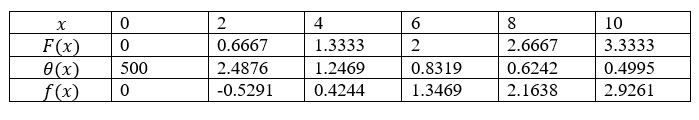
\includegraphics[height=25mm]{Programs/Program 3/progc820474fig1.PNG}
 \caption{Results from Manual Force and Angle Computation in Example 1}
 \label{f:Table 1}
\end{figure}
\par \medskip
Then I calculated the h-value (step size) as 
$h=\frac{(x_i-x\textsubscript{i-1})}{n}$, n = number of points
\par \medskip
      By plugging in the points, I got h=2.  Then, the value of the work using Simpson’s 3/8th Rule was:
$W \approx \frac{3h}{8} [f(x_0 )+3f(x_1 )+2f(x_2 )+3f(x_3 )+3f(x_4 )+f(x_5 )]$
\par \medskip
$W \approx 9.5396 Nm$
\par \medskip
When these values are plugged into the formula above, we get that W is approximately 9.5396.  When calculating the exact value, I plugged in the values a, b, force, and angle values into the original integral defined in Steven Chapra and Raymond Canale’s work [CC10]: 
$W\textsubscript{exact}=\int_{0}^{10}\! \frac{x}{3}*cos(\frac{5}{x+0.1}) \, \mathrm{d}x \approx 9.9083 Nm$
It can be seen that the values are pretty close but not equal. This notion is because I only used n=5 points. If I increase the number of points, the error will reduce. Table 2 presents the value of the work obtained by different number of points, and it can be seen that as the number of points increases, the value of the approximation approaches to the exact value:
\par \medskip
 \begin{figure}[!ht]
\centering  %centering can be used to center the image
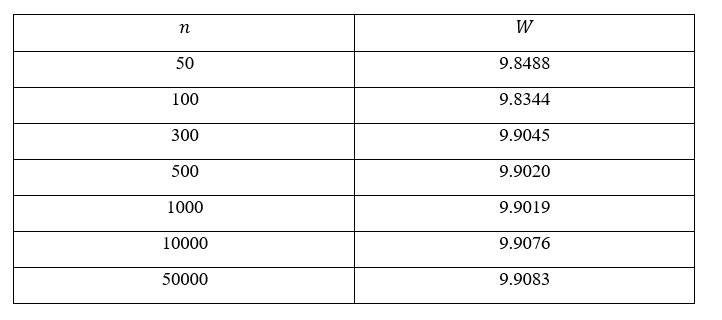
\includegraphics[height=55mm]{Programs/Program 3/progc820474fig2.PNG}
 \caption{Results of Work from Different Plot Points in Example 1}
 \label{f:Table 2}
\end{figure}
\par \medskip
Similar results can be shown using the Trapezoidal Method as well.  By using the same $F(x)$, $q(x)$, a, and b values as the previous example, the x-value can be defined as $x=[0 1.4286 2.8571 4.2871 4.2857 5.7143 7.1429 8.5714 10]$.  By evaluating the force and angle at each point x, Table 3 shows the values given:
\par \medskip
 \begin{figure}[!ht]
\centering  %centering can be used to center the image
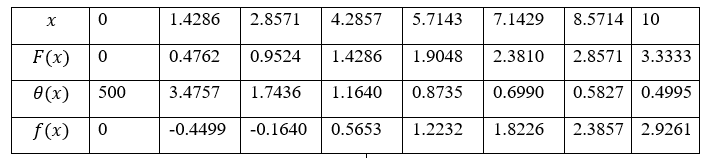
\includegraphics[height=35mm]{Programs/Program 3/progc820474fig3.PNG}
 \caption{Results from Manual Force and Angle Computation in Example 2}
 \label{f:Table 3}
\end{figure}
\par \medskip
Using the trapezoidal method, defined as,
$Y \approx \frac{h}{2} (f(x\textsubscript{0})+2\sum_{i=1}^{n-1} f(x\textsubscript{i})+f(x\textsubscript{n)})$,
     we get that 
$W \approx 9.7799 Nm$
     The exact value is:
$W\textsubscript{exact}=\int_{0}^{10}\! \frac{x}{3}*cos(\frac{5}{x+0.1}) \, \mathrm{d}x \approx 9.9083 Nm$
\par \medskip
      In the case of these force and angle functions, it is clear that the trapezoidal method came the closest to calculating the exact value.  In this case, the advantage of the Trapezoidal Method is that, as the number of points increases, the error reduces at a higher rate than the Simpson’s Rule. For a different numbers of points, we have that the approximation and the error is represented in Table 4:
\par \medskip
 \begin{figure}[!ht]
\centering  %centering can be used to center the image
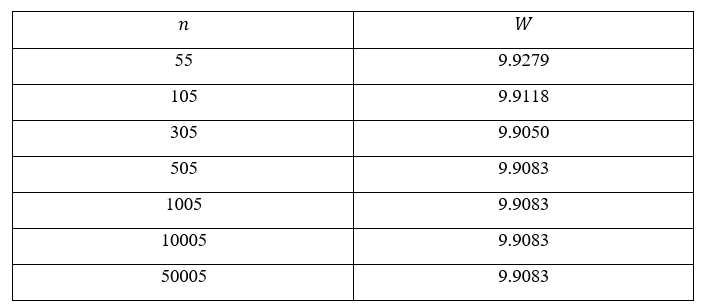
\includegraphics[height=55mm]{Programs/Program 3/progc820474fig4.PNG}
 \caption{Results of Work from Different Plot Points in Example 2}
 \label{f:Table 4}
\end{figure}
\par \medskip
Though we came closer using the Trapezoidal Method, comparing the table above with the table from Simpson’s Method, it can be seen that, for Simpson’s 3/8th Rule, the calculations obtained had an approximation equal to the exact value with 50000 points. In comparison, the Trapezoidal Method just needed 505 points.  For these functions, it makes the Trapezoidal Method more accurate in this case.
\par \medskip
When coded, we get the following result:
\par \medskip
x = linspace(0, 10, 1005);
\par \medskip
F = x./3;
\par \medskip
theta = 5./(x+0.01);
\par \medskip
[flag, approx] = progc123456(x, F, theta)
\par \medskip
flag = 3
\par \medskip
approx = 9.908934855664397
\par \medskip
\par \medskip
As it can be seen, the approximation for these values matches along with the indication of flag 3 to indicate the Trapezoidal rule was used to calculate this code, respectively.
\par \medskip
Other examples can be tested using this code as well.   We can test the code with a case when F is constant and theta is always zero.  This case represents a normal case for a constant force parallel to the motion.  For example. F = 10, and d = 30. Then the work done is $W = Fd = (10)(30) = 300$.  In the code, I defined a vector from 0 to 30, making 100 points between 0 and 30.  Then, I defined a vector such that F is a constant throughout the entire interval.  Then, I defined theta such that it is always zero and ran the program.  The code showed:
\par \medskip
x = linspace(0, 10, 8);
\par \medskip
n = length(x);
\par \medskip
F = 10*ones(1, n);
\par \medskip
theta = zeros(1, n);
\par \medskip
[flag, approx] = progc820474(x, F, theta)
\par \medskip
flag = 3
\par \medskip
approx = 100
\par \medskip
\par \medskip
Though this approximation is off from the exact value, it is the right approximation using Trapezoidal Method.  
\par \medskip
Another example is defining the vectors F, x, and theta within the command line and testing to see which method was used to calculate the approximation.  Using $x = [0, 5, 10, 15, 20, 25, 30]$, $F=[0, 9.0, 12.1, 13.7, 14.2, 14.4, 17.1]$, and $theta = [0.5, 0.6, 0.75, 0.8, 1.2, 1.5, 1.62]$, the code outputs the following:
\par \medskip
x = [0, 5, 10, 15, 20, 25, 30];
\par \medskip
F = [0, 9.0, 12.1, 13.7, 14.2, 14.4, 17.1];
\par \medskip
theta = [0.5, 0.6, 0.75, 0.8, 1.2, 1.5, 1.62];
\par \medskip
[flag, approx] = progc123456(x, F, theta)
\par \medskip
flag = 2
\par \medskip
approx = 1.598591369577752e+02
\par \medskip
\par \medskip
As shown in the code above, Simpson’s 3/8th Rule was used to calculate the approximation of the vectors x, F, and theta given in the command window.  These values can also be defined within the program or in the function call.  This calculation shows that Simpson’s 3/8th Rule was used effectively and correctly.
\par \medskip
From the above example call functions, I concluded that:
\par \medskip
1. The approximations found by the function for the examples done by hand are the same.
\par \medskip
2.  When the input values are outside the interval, the algorithm provides the desired results.
\par \medskip
3. When the input values are valid, the algorithm goes through each condition to decide whether Simpson’s 3/8th Rule or Trapezoidal Rule is computed.
\par \medskip
4.  When computed, the algorithm prints out the appropriate flag and approximation value.
\par \medskip
Thus, the code and the calculations by hand prove that the program is producing accurate calculations.

}




% ---------------------------------------------------
% Anything after the \end{document} will be ignored by the typesetting.
% ----------------------------------------------------

\end{document}